\documentclass{article}     
\usepackage[utf8x]{inputenc}
\usepackage[english,russian]{babel}
\usepackage[section]{placeins}
\usepackage{upgreek}
\usepackage{graphicx}
\usepackage{wrapfig}
\usepackage{amsmath}
\graphicspath{{images/}}

\textheight 24.5cm % 29.7-2-2=25.7
\textwidth 17cm % 21-2.5-1.5=17.0
\hoffset -0.04cm %2.5-2.54=-0.04 слева 3см
\voffset -0.54cm %2-2.54=0.54 сверху 2см
\oddsidemargin 0cm
\headheight 0cm
\headsep 0cm
\topmargin 0cm



\begin{document}
\begin{titlepage}
\begin{center}
{\bf САНКТ-ПЕТЕРБУРГСКИЙ ГОСУДАРСТВЕННЫЙ УНИВЕРСИТЕТ\\
МАТЕМАТИКО-МЕХАНИЧЕСКИЙ ФАКУЛЬТЕТ\\}
\end{center}

\vspace{2cm}
 \begin{center}
  \Huge{\bf{Построение профилей линий в спектрах
   звезд\\ типа 
   TTau и Ae/Be Хербига }}
 \end{center}

\vspace{2cm}

\large
 \hspace{8cm}\parbox{8cm}{	

{\bf Курсовая работа}\\
студента 13C04-ММ группы\\
Д.В.\,Дмитриева  
\vspace{1cm}

{\bf Научный руководитель}\\
 д.ф.-м.н, профессор РАН\\ В.П.\,Гринин \\ 
}

\vfill 
\begin{center}
Санкт-Петербург

2017
\end{center}

\end{titlepage}
\newpage
\begin{abstract}
Данная работа посвящена разработке алгоритма расчета эмиссионного спектра молодой звезды и является развитием предыдущей курсовой работы \cite{kurs}. В модель добавлен более аккуратный способ рассчета магнитоферной аккреции (см. раздел Магнитосферная аккреция), а также промоделирована линия He 10830\AA , наблюдаемая в спектрах звезд типа Ае/Be Хербига и Т Тельца.
\end{abstract}
\tableofcontents



\newpage


\numberwithin{equation}{section}

\section{Введение}
Тип T Тельца и Ае/Ве Хербига -- это молодые звезды, ещё не достигшие главной последовательности. Они отличаются массами, эффективной темпертарурой и скоростями вращения: звезды типа Т Тельца ($T_{ef} \approx$ 4000 K) имеют массы в интервале от 0.2 до 2 $M_\odot$; их средняя скорость вращения равна примерно 15 км/с 
(см. обзор Петрова \cite{petrov}.). Звезды Ае/Ве Хербига имеют более высокие эффективные температуры ($T_{ef} \approx$ 8000-30000 K). Их массы заключены в пределах от 2 до 10 $M_\odot$. Скорости вращения достигают значений порядка 100-200 км/с (см. обзор \cite{waters98}). \\
Многие молодые звезды окружены околозвездными газопылевыми диски, в которых формируются планетные системы. Вещество дисков аккрецирует на звезды. 
Важную роль в этом процессе играет крупномасштабное магнитное поле молодой звезды (см. например, Хартманн и др. \cite{hartman94}). У звезд типа Т Тельца оно достигает значений порядка 1-2 кГс (см. обзор \cite{petrov} и цитированные там работы). У звезд Ае/Ве Хербига магнитное поле заметно меньше, что объясняют отсутствием у горячих звезд конвективной оболочки. \\

Исследования показывают, что основной вклад в эмиссионные спектры молодых звезд дают две области околозвездного пространства: 
магнито-центробежный ветер, стартующий с поверхности аккреционного диска, и магнитосфера звезды. У звезд типа Т Тельца доминирует вклад магнитосферы и прилегающей к ней области (Х-ветер, Шу и др. \cite{shu94}), тогда как у звезд Ае/Ве Хербига важную роль 
в формировании эмиссионного спектра играет дисковый ветер (Гринин и Тамбовцева \cite{grinin11}). \\
В этом году алгоритм, описанный в работе прошлого года, применялся к ветру завезд типа Ае/Ве Хербига (см. ниже), кроме того в алгоритм была добавлена более аккуратная модель аккреции (см. раздел Магнитосферная аккреция). Такая модель аккреции использовалась в работе Хартманна 1994 года (\cite{hartman94})


\section{Линия He 10830 \AA\ в спектрах звезд типа Ae/Be Хербига}

В спектрах звезд Ae/Be Хербига наблюдается линия Не 10830 \AA, которая происходит при переходе с уровня $3^3P$ на $2^3S$ . Нижний уровень этого перехода матастабильный, что приводит к накапливанию электронов на нем. Профили этой линии предполагают наличие горячего ветра, возникающего в полярных областях звезды. Были рассмотренны две модели ветра. Первая предполагает электронную температуру в ветре порядка $10^6 K$. При таких условиях практически весь газ будет ионизован столкновениями с электронами, что приводит к небольшой оптической толщине в линии. Вторая модель предполагает "теплый" ветер с температурой порядка $10^4 K$. Заселение нижнего уровня в результате ионизаций атомов гелия рентгеновским излучением и последующих рекомбинациях. Рентгеновское излучение возникает в горячих аккреционных пятнах на поверхности звезды и в ее короне. Схематически модель геометрии ветра представлена на Рис. 1. 

\begin{figure} [h]
    \centering
    \includegraphics[width=0.6\textwidth]{Hot_wind}
    \caption{Схематическое представление модели теплого ветра. 1 -- аккреционный диск, 2 -- звезда, 3 -- аккрецирующий газ, в точках его падения на зезду образуются горячие пятна, 4 -- область ветра}
\end{figure}

В такой модели возможно получить большую оптическую толщину, что приводит к образованию линии.  \\
Ветер моделировался конусом с углом раствора $\theta=45^\circ$ и стратовым радиусом $3.7$ радиуса звезды ($1.3\times 10^{12}$ см). Ось конуса составляет с лучом зрения угол $i$.  Начальная скорость ветра $v_0$ принималась равной 30 км/с, конечная $v_\infty$ --- 400 км/с. Зависимость скорости ветра от расстояния до звезды определялась формулой  

\[
v = v_0 + \left(v_{\infty} - v_0\right)\left(1 - \frac{1}{r}\right)^\beta
\] 

где параметр $\beta = 1.8$. Это классическая апроксимация ветров, возникающих в оболочках звезд (см. \cite{castor79}) \\
Ниже приводятся результаты для различных электронных температур ветра. Состояния ионизации и населенности уровней рассчитывались Т.А. Ермолаевой с помощью пакета CLOUDY. Более подробно по этому разделу см. работу \cite{tamara}.\\
Стоит отметить, что в этом пакете не учитывается движение газа, поэтому населенности верхнего уровня рассматриваемого перехода, полученные с помощью этого пакета не верны, так как этот уровень заселяется радиационно с нижнего. Нижний же уровень заселяется при рекомбинациях свободных электронов. Поэтому функция источника рассчитывалась в приближении Соболева, предполагая, что линия резонансная. На Рис. 2 и 3 представлены рассчитанные таким путем профили линии Не 10380 \AA. (Детали расчетов см. в разделе 5.2 Приложения). Похожие профили этой линии наблюдаются в спектрах многих звезд типа АеВе Хербига (см. например, \cite{cauley}).

\begin{figure} [h]
    \centering
    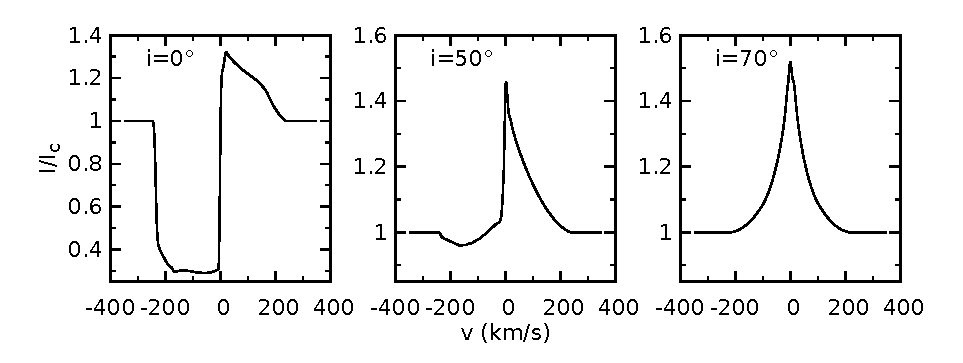
\includegraphics[width=1\textwidth]{prof}
    \caption{Теоретические профили линии при $T_e=9000K$ и различных углах $i$}
\end{figure}

\begin{figure} [h]
    \centering
    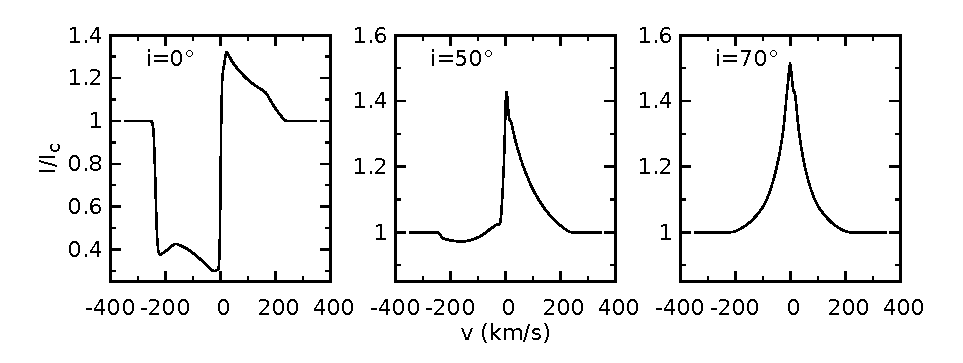
\includegraphics[width=1\textwidth]{prof1}
    \caption{Теоретические профили линии при $T_e=15000K$ и различных углах $i$}
\end{figure}

\section{Магнитосферная аккреция}

Из-за сильного магнитного поля, газ падает на звезду не в плоскости диска, а в какой-то моммент отклоняется, и начинает двигаться вдоль магнитно-силовых линий. Мы считаем, что магнитное поле настолько сильное, что падающий газ никак не воздействует на него \cite{hartman94}. В работе предыдущего года предпологалось, что газ падает на звезду радиально, внутри области, ограниченной двумя конусами. Такое предположение оправдано тем, что самый горячий газ находится рядом со звездой, где магнитно-силовые линии практически прямые. Более точная модель предполагает, что магнитное поле звезды имеет дипольную геометрию, и газ находится в области, ограниченной двумя поверхностями вида $r = r_m\sin^2\theta$, где $\cos \theta = \frac{z}{r}$, где $r$ - расстояние до звезды, а ось $z$ направлена вдоль оси магнитного диполя. Скорость газа в таком случае тоже направлена по касательной к соответствующей поверхности такого вида \cite{hartman94}.

Для того, чтобы рассчитать профиль, необходимо рассчитывать проекцию скорости на луч зрения в любой точке области. Если предположить, что вещесво падает с расстояния $r_o$, то модуль скорости будет равен

\[
v = v_{esc}\sqrt{\left(\frac{1}{r} - \frac{1}{r_o}\right)}
\]

Где $r$ измеряется в радиуах звезды, $v_{esc}$ -- скорость убегания с поверхности звезды, а .  Направление же скорости можно определить, высчитав направление нормали к поверхности на которой лежит интересующая нас точка. Тогда можно определить проекцию скорости на луч зрения. \\

Как уже было сказано выше, область ограничена двумя поверхностями: $r=r_{in}\sin^2 \theta$ и $r=r_{out}sin^2 \theta$. На Рис.4 представлено схематичное изображение области. 

\begin{figure} [h]
    \centering
    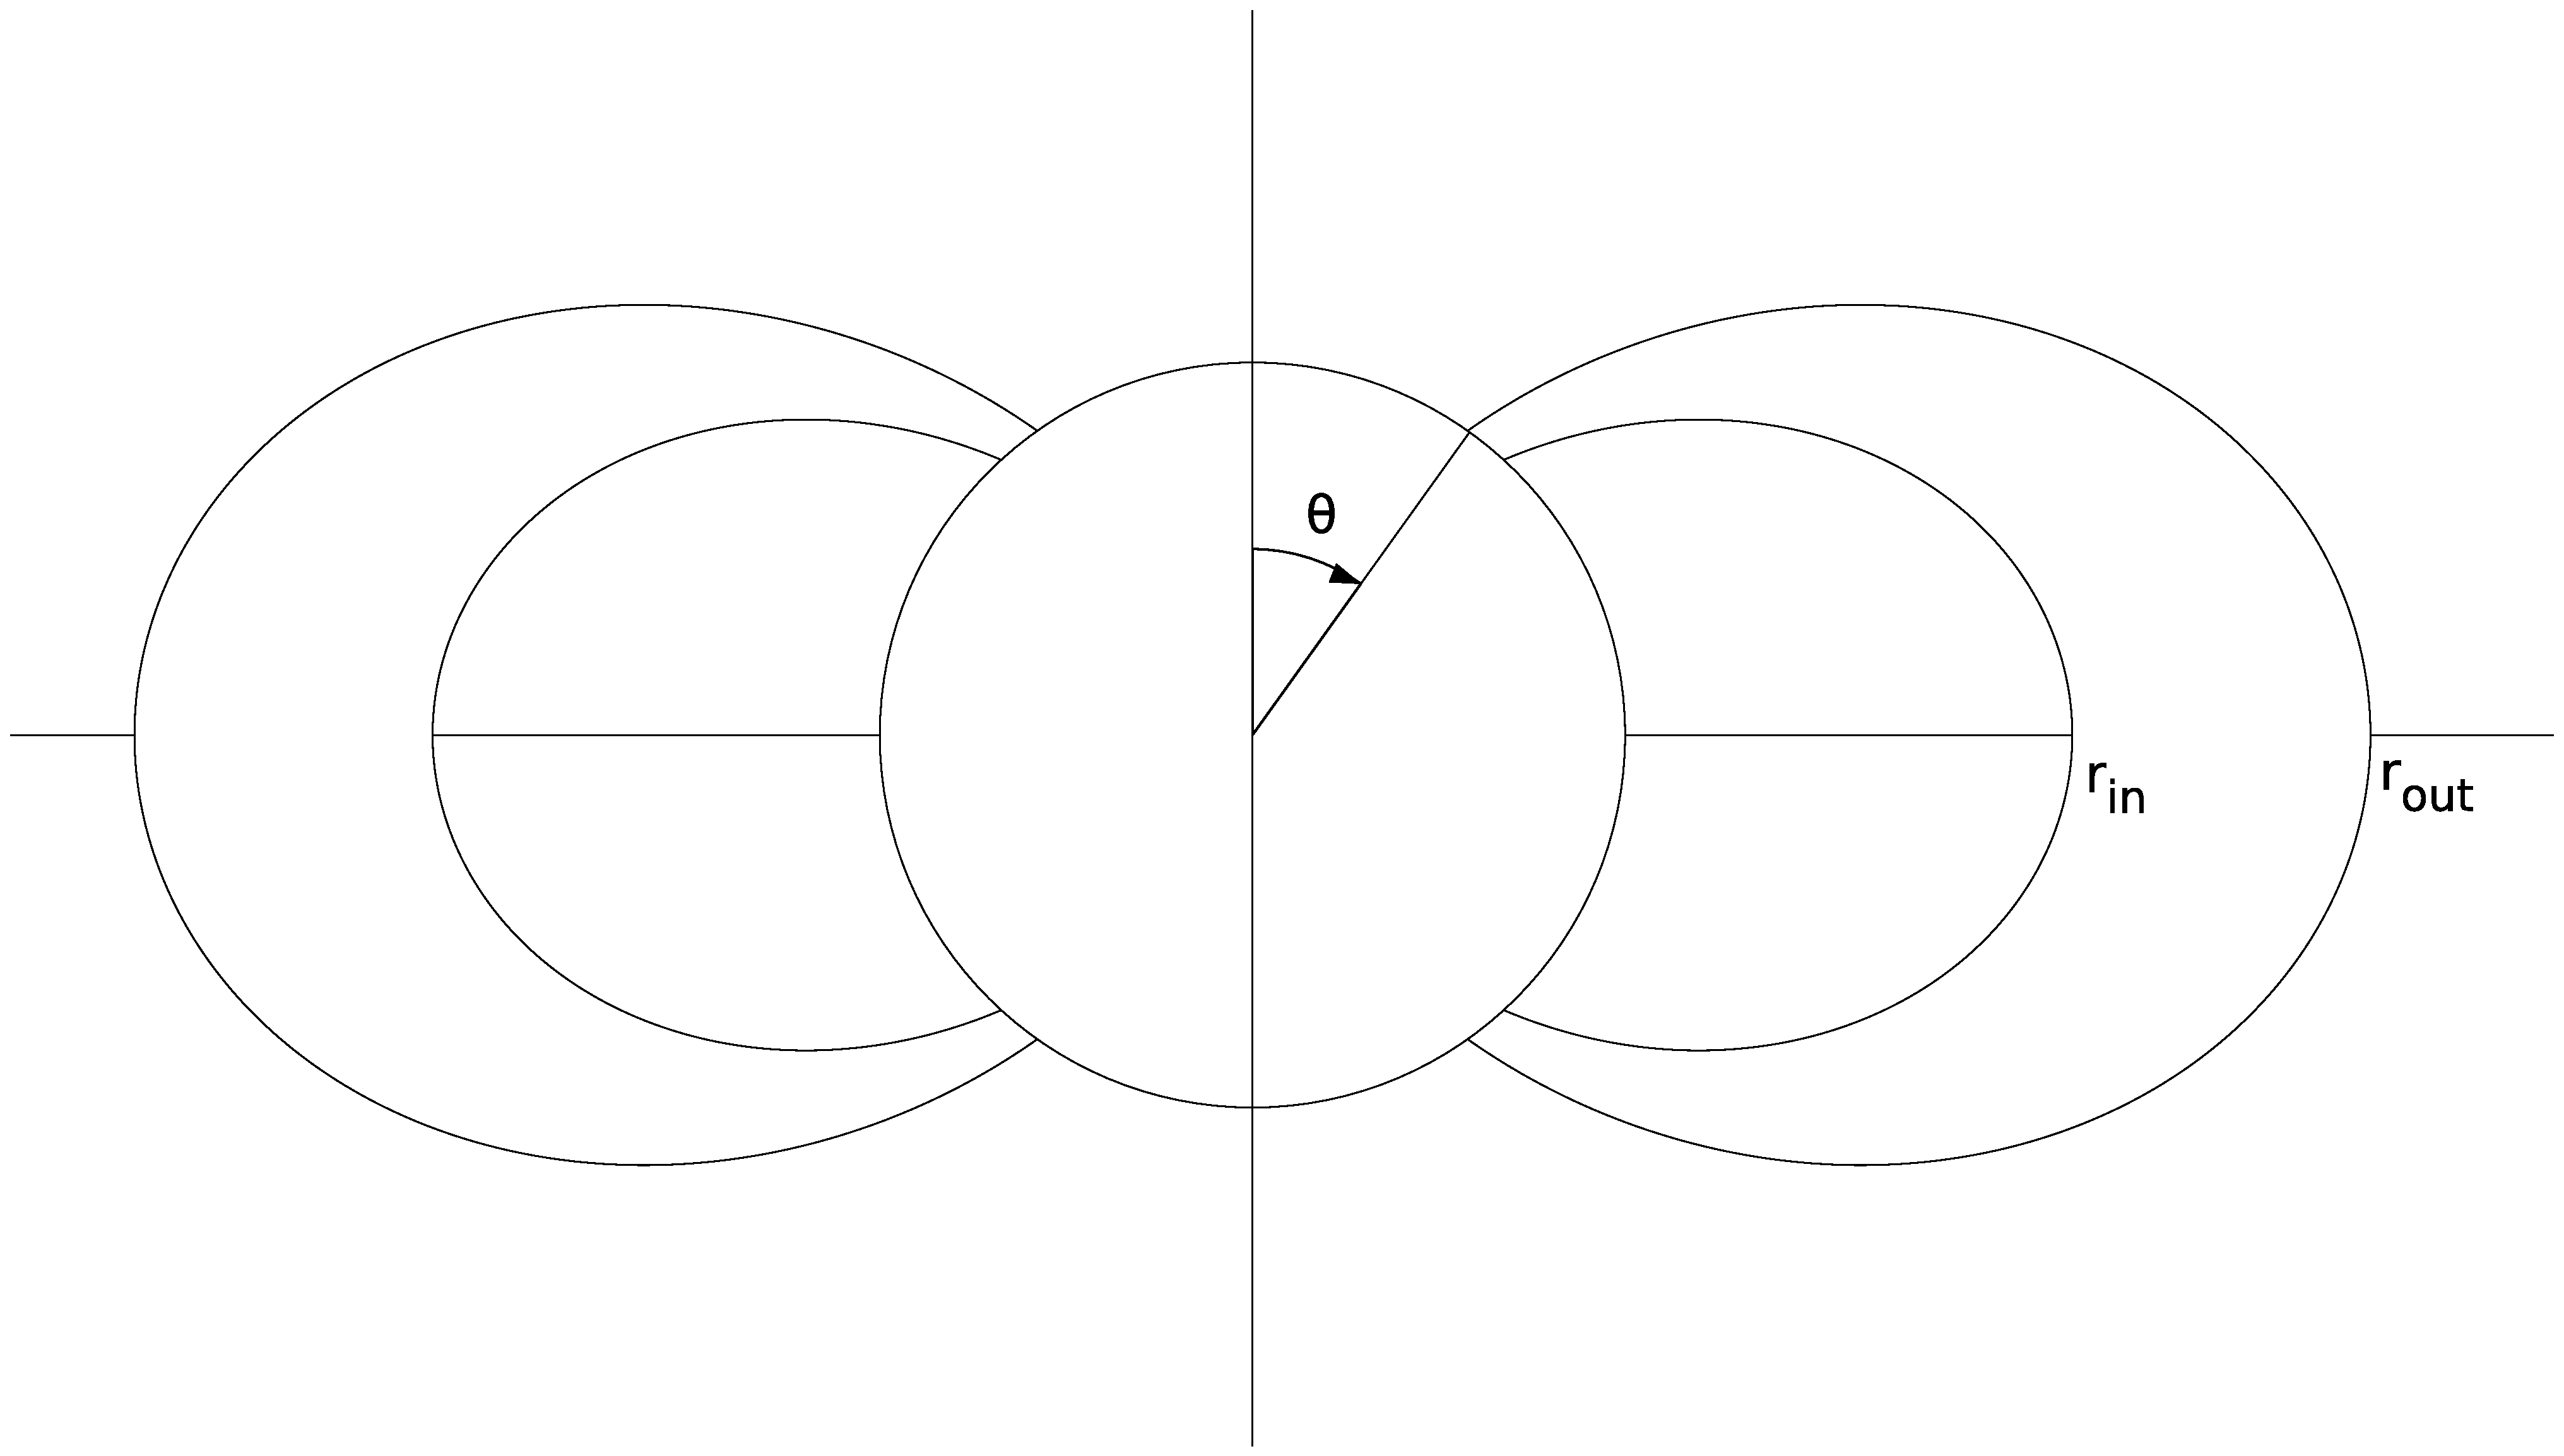
\includegraphics[width=0.65\textwidth]{accr}
    \caption{Область аккреции}
\end{figure}

\subsection{Теоретические профили водородных линий без вращения}
Далее (Рис. 5, 6 и 7) представлены профили линий $H_\alpha$, $H_\beta$ и $H_\gamma$, полученные параметрах $r_{in}=2.2$ и $r_{out}=3.0$. Рассчет температуры внутри магнитосферы представляет собой очень сложную задачу. Ниже использован температурный режим, определяемый формулой:  

\[
T = T_0 r^{-\frac{1}{3}}
\] 

Где $T_0$ - значение температуры аккрецирующего газа вблизи поверхности звезды. Ниже принято $T_0 = 8000 K$. Такое распределение температуры в магнитосфере звезды в первом приближении согласуется с температурным режимом, принятым в работе Хартманна и др. \cite{hartman94} Параметры звезды: $T_{eff}=10000K$, $R=2.6R_\odot$, $M=4.0M_\odot$. \\

Профили рассчитывались для различных углов наклона оси диполя к лучу зрения (различных $i$). Расчеты населенностей были выполнены Л.В.Тамбовцевой в приближении Соболева, с использованием алгоритма, описанного в работах Гринина и Катышевой \cite{grinin80} и Гринина и Мицкевича \cite{grinin90}.

\begin{figure} [!htb]
    \centering
    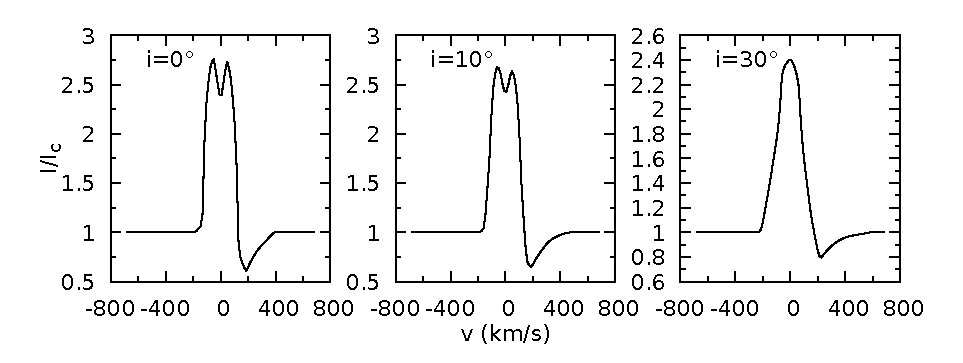
\includegraphics[width=0.85\textwidth]{Ha_0_10_30}
    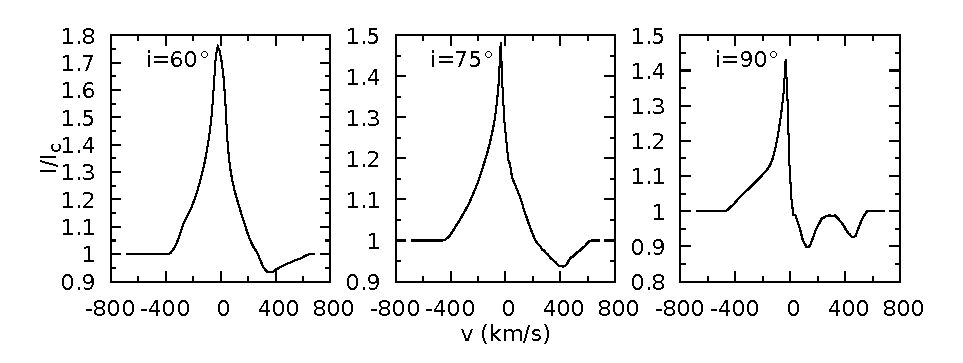
\includegraphics[width=0.85\textwidth]{Ha_60_75_90}
    \caption{Теоретические профили линии $H_\alpha$ для различных углов наклона к лучу зрения}
\end{figure}

\begin{figure} [!htb]
    \centering
    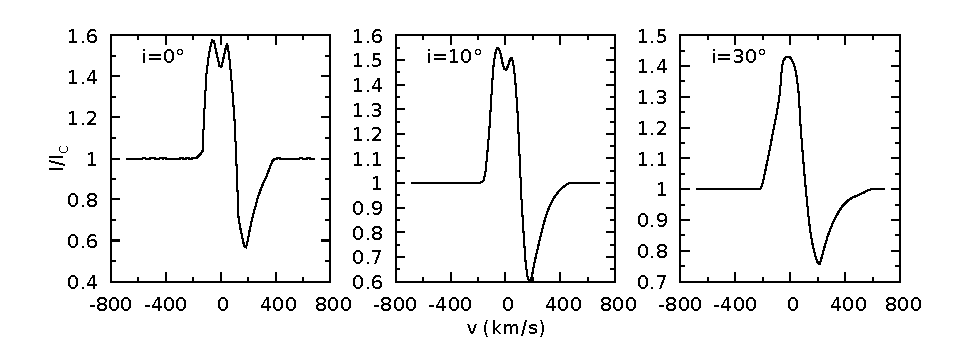
\includegraphics[width=0.85\textwidth]{Hb_0_10_30}
    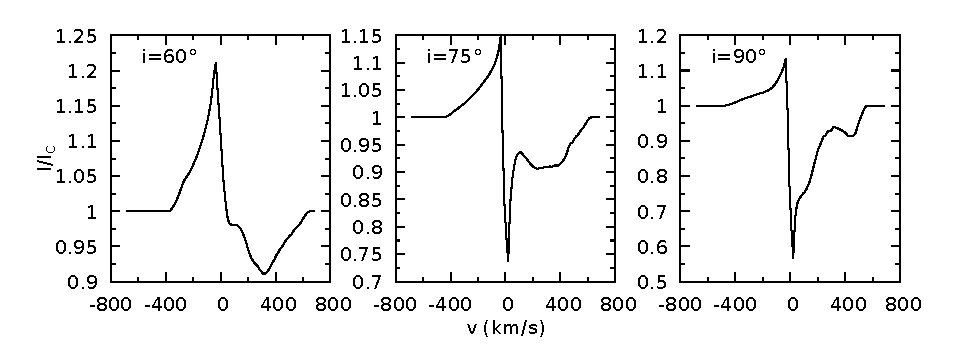
\includegraphics[width=0.85\textwidth]{Hb_60_75_90}
    \caption{Теоретические профили линии $H_\beta$ для различных углов наклона к лучу зрения}
\end{figure}


\begin{figure} [!htb]
    \centering
    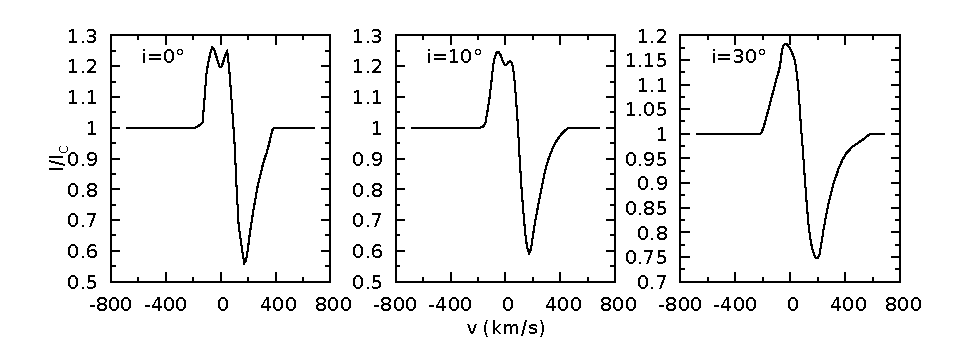
\includegraphics[width=0.85\textwidth]{Hg_0_10_30}
    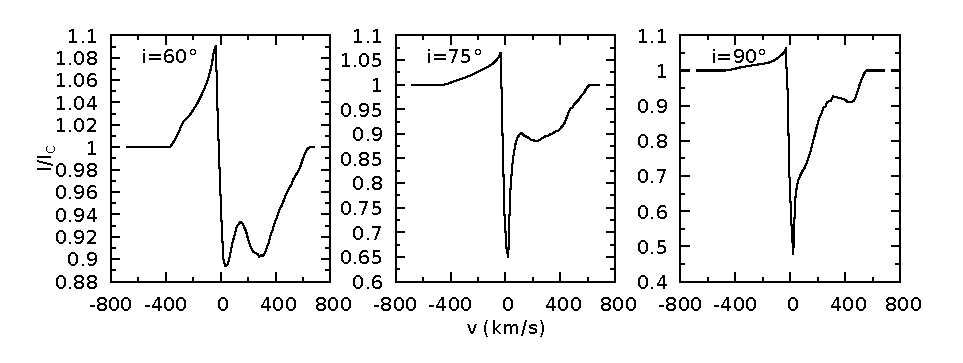
\includegraphics[width=0.85\textwidth]{Hg_60_75_90}
    \caption{Теоретические профили линии $H_\gamma$ для различных углов наклона к лучу зрения}
\end{figure}

\subsection{Вращение магнитосферы: переменность профилей}

В данном разделе рассматривается случай, когда ось диполя не сонаправлена с осью вращения звезды. Предполагается, что область аккреции вращается твердотельно, вместе со звездой (ее магнитным полем). Рассматривался угол между ними в 15 градусов. Ниже на Рис 8 и 9 приведены профили для фаз ($\psi$) от 0 до 180 градусов. Профиль для $psi$ от 180 до 360 градусов практически повторяет) профиль с $psi = 360-180$ градусов. Для того, чтобы профили с разными $psi$ не накладывались друг на друга, к каждому профилю прибавлялось $\frac{\psi}{100}$. На Рис.10 показаны те же профили, только без этой прибавки, чтобы лучше был виден диапазон переменности. Скорость вращения на экваторе - 30 км/с. \\


\section{Заключение}

В этом году была успешно промоделирована линия Не 10830 \AA , а также добавлена новая модель аккреции, более аккуратно описывающая явления, происходящие в оболочках звезд типа Т Тельца и Ае/Ве Хербига.

\begin{figure} [!htb]
 	\centering
    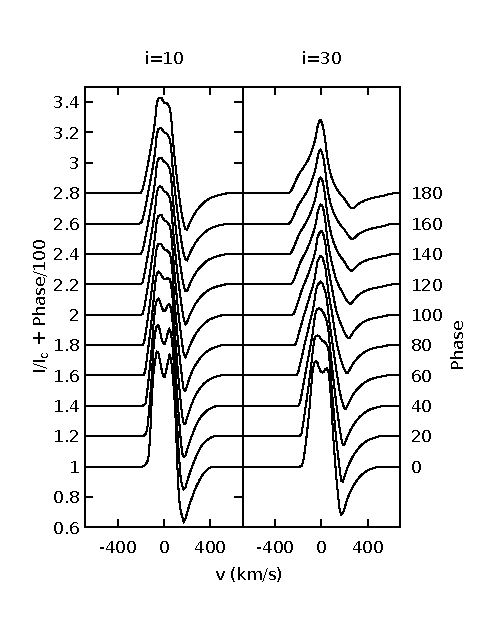
\includegraphics[width=1.0\textwidth]{rot_all_10_30}
    \caption{Переменность профилей линии $H_\beta$}
\end{figure}


\begin{figure} [!htb]
 	\centering
    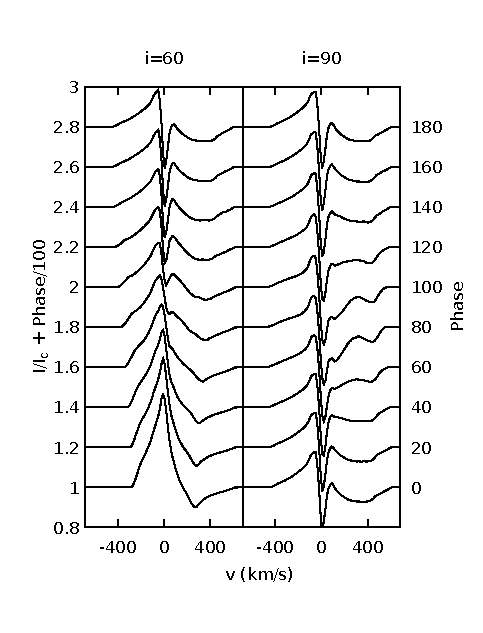
\includegraphics[width=1.0\textwidth]{rot_all_60_90}
    \caption{Переменность профилей линии $H_\beta$}
\end{figure}

\begin{figure} [!htb]
    \centering
    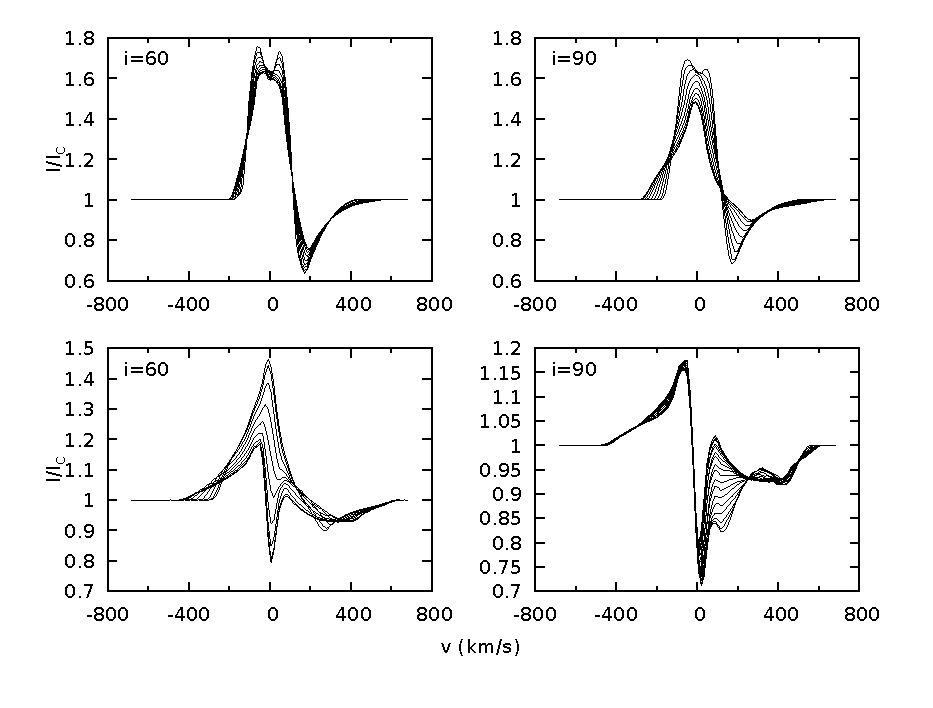
\includegraphics[width=1.0\textwidth]{rot_10_30_60_90}
    \caption{Переменность профилей линии $H_\beta$}
\end{figure}

\pagebreak

\section{Приложение: немного из работы прошлого года}

Ниже приводятся некоторые формулы из курсовой работы прошлого года, использованные при расчетах профилей спектральных линий.

\subsection{Ориентация оси магнитного диполя в пространстве}

Ориентация магнитного диполя задается трямя углами:
\begin{itemize}
\item $i$ -- угол между лучом зрения и осью вращения звезды
\item $\psi$ -- фазовый угол. Угол между плоскостью "луч зрения - ось вращения" и "ось диполя - ось вращения"
\item $\alpha$ -- угол между осью вращения и осью диполя
\end{itemize}

Положение оси задается именно таким образом для того, чтобы было удобно моделировать твердотельное вращение области -- можно просто варьировать угол $psi$. Для того, чтобы упростить вычисления вводится следующая система координат: 
\begin{itemize}
\item ось z направляется вдоль луча зрения, по направлению к наблюдателю
\item ось y задается в плоскости "ось диполя - луч зрения" перпендикулярно оси z? так, чтобы ось диполя лежала между положительными направлениями обоих осей
\item ось x вводится перпендикулярно y и z так, чтобы оси составляли правую тройку векторов
\end{itemize}

Чтобы учесть вращение области необходимо знать вектор угловой скорости в новой системе координат. Можно вычислить, что

\[
\begin{aligned}
\omega_x & = \omega \sin i \sin \alpha \sin \psi / \sin \theta \\
\omega_y & = \omega \sin i (\cos \alpha \sin i - \cos i \sin \alpha \cos \psi) \\
\omega_z & = \omega \cos i \\
\\
\theta & = \arccos (\cos i \cos \alpha + \sin i \sin \alpha \cos \psi)
\end{aligned}
\]

Где $\theta$ -- угол между лучом зрения и осью диполя, а $omega$ -- угловая скорость области.

\subsection{Рассчет профиля линии}

В общем случае профиль линии задается формулой

\begin{equation}
I_{\nu} = \int \limits_{S} I_{xy}(\nu) dS
\end{equation}

Где $S$ - площадь проекции области, в которой происходит излучение, на плоскость $XY$ (ось $z$ направлена на наблюдателя), а $I_\nu$ - интенсивность излучения в линии  на частоте $\nu$ 

Рассмотрим $I_{xy}$
\begin{equation}
I_{xy}(\nu) =  \int \limits_{z_0}^{z_k} S_{ul}k_{lu}e^{-\tau}dz
\end{equation}
\begin{equation}
\tau = \int \limits_z^{z_k} k_{lu}dz
\end{equation}
\begin{equation}
S_{ul} = \frac{2h\nu_0^3}{c^2}\left(\frac{n_l}{n_u} \frac{g_u}{g_l} - 1 \right)^{-1}
\end{equation}
\begin{equation}
k_{lu} = 0,02654f_{lu}\alpha(\nu, z)n_l\left(1 - \frac{g_l}{g_u}\frac{n_u}{n_l}\right)
\end{equation}
\begin{equation}
\alpha(\nu, z) = \frac{1}{\sqrt{\pi} \Delta\nu_D} \exp\left( -\left[ \frac{\nu}{\Delta\nu_D} - \frac{v_z(z)}{u}\right]^2\right)
\end{equation}

Где $S(z)$ - функция источника, $k(\nu, z)$ - коэффициент поглощения, $\nu_0$ - центральная частота линии, $u$ - тепловая скорость, $\Delta\nu_D$ - доплеровская ширина линии, $v_z(z)$ - лучевая скорость вещества в точке $(x, y, z)$.

Населенности уровней задаются извне. 

Излучение в континууме задается формулой Планка.

\begin{equation}
I_c = \frac{2h\nu^3}{c^2}\frac{1}{\exp\left(\frac{h\nu}{k_bT_s}\right)-1}
\end{equation}

Где $T_s$ - эффективная температура звезды. Теперь можно рассчитать профиль $r_{\nu}$

\begin{equation}
r_{\nu} = \frac{I_\nu + I_{\tau}(\nu)}{I_c \pi R_\ast^2}
\end{equation}

Где $I_{\tau}$ учитывает поглощение излучения звезды в области

\begin{equation}
I_{\tau}(\nu) = \int \limits_{S_\ast} I_c e^{-\tau} dS
\end{equation}

Где $S_\ast$ - проекция звезды на картинную плоскость, а $\tau$ - оптическая толщина на всем луче.

\begin{thebibliography}{99}
\bibitem{castor79} Castor J. I., Lamers H. J. G. L. M., 1979, ApJS, 39, 481
\bibitem{petrov} П.П. Петров, Астрофизика
\bibitem{waters98} Waters, Waelkence, Ann. Rev. Astron. Astrophys. 1998 
\bibitem{hartman94} L. Hartmann et al. ApJ, 1994
\bibitem{shu94} F. Shu et al. ApJ, 1994
\bibitem{grinin11} В.П. Гринин, Л.В. Тамбовцева, Астрон. Ж. 2011
\bibitem{kurs} Д.В.Дмитриев, Курсовая работа, 2016 год, н. рук. В.П. Гринин
\bibitem{tamara} Formation of the line He I 10830 {\AA} in biconical winds of Herbig Ae/Be stars, T.A. Ermolaeva, V.P. Grinin, D.V. Dmitriev, Труды Международной астрономической конференции "STARS: FROM COLLAPSE TO COLLAPSE", САО РАН, 2016, в печати. 
\bibitem{grinin80} В.П Гринин, Н.А. Катышева, Изв. Крымск. астрофиз. обсерв. 62, 59 (1980).
\bibitem{grinin90} В.П. Гринин, А.С. Мицкевич, Астрофизика, 32, 383 (1990).
\bibitem{cauley} Cauley and Johns-Krull, Astrophysical Journal, 797, 112, 2014

\end{thebibliography}

\end{document}